\documentclass[10pt,aspectratio=169]{beamer}

\usetheme[progressbar=frametitle]{metropolis}
\usepackage{appendixnumberbeamer}
\usepackage[noend]{algpseudocode}
\usepackage{algorithmicx}
\usepackage{booktabs}
\usepackage[scale=2]{ccicons}

\usepackage{pgfplots}
\usepgfplotslibrary{dateplot}

\usepackage{xspace}
\newcommand{\themename}{\textbf{\textsc{metropolis}}\xspace}
\usepackage[orientation=landscape,size=custom,width=16,height=9,scale=0.5,debug]{beamerposter}%修改比
\usepackage{tikz}
\usepackage[linesnumbered, ruled]{algorithm2e}
\SetKwRepeat{Repeat}{repeat}{until}%
\usepackage{verbatim}
\usetikzlibrary{arrows,shapes}

\title{Paper Presentation}
\subtitle{Adversarial training methods for semi-supervised text classification}
% \date{\today}
\date{\texttt{Nov 12, 2019}}
\author{\texttt{Baodi Shan}}
% \institute{Center for modern beamer themes}
%\titlegraphic{\hfill\includegraphics[height=3cm]{matching.png}}

\begin{document}
\pgfdeclarelayer{background}
\pgfsetlayers{background,main}






\maketitle

\begin{frame}[fragile]{Something Embarrassing}
	\begin{columns}[onlytextwidth]
		\column{.4\textwidth}
		
		\begin{figure}
			
\includegraphics[width=1.2\linewidth]{gg.jpg}
		\end{figure}
		
	\end{columns}
\end{frame}




\begin{frame}{Table of Contents}
	\setbeamertemplate{section in toc}[sections numbered]
	\tableofcontents[hideallsubsections]
\end{frame}

%\input
\section{Introduction}

\begin{frame}[fragile]{Last Week}
	\begin{columns}[onlytextwidth]
		\column{.4\textwidth}
		
		\begin{itemize}
			\item Have admiration for him
			\item 
			\item 
		\end{itemize}
		
		\column{.6\textwidth}
		
		\begin{figure}
			
\includegraphics[width=.5\linewidth]{peifu.jpg}
		\end{figure}
		
	\end{columns}
\end{frame}


\begin{frame}[fragile]{Last Week}
	\begin{columns}[onlytextwidth]
		\column{.4\textwidth}
		
		\begin{itemize}
			\item Have admiration for him
			\item Confused
			\item 
		\end{itemize}
		
		\column{.6\textwidth}
		
		\begin{figure}
			
\includegraphics[width=.5\linewidth]{mengbi.jpg}
		\end{figure}
		
	\end{columns}
\end{frame}

\begin{frame}[fragile]{Last Week}
	\begin{columns}[onlytextwidth]
		\column{.4\textwidth}
		
		\begin{itemize}
			\item Have admiration for him
			\item Confused
			\item In Despair
		\end{itemize}
		
		\column{.6\textwidth}
		
		\begin{figure}
			
\includegraphics[width=.5\linewidth]{juewang.jpg}
		\end{figure}
		
	\end{columns}
\end{frame}



\begin{frame}[fragile]{Story About Adversarial training}
	\begin{columns}[onlytextwidth]
		\column{.4\textwidth}
		
		\begin{figure}
			\caption{Dog}
			
\includegraphics[height=0.5\textheight]{fig0.jpg}
		\end{figure}
	
		\column{.5\textwidth}
		\begin{figure}
			\caption{What?}
			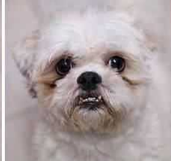
\includegraphics[height=0.5\textheight]{fig2.jpg}
		\end{figure}
	
		\end{columns}
		\begin{itemize}
			\item Why?
		\end{itemize}
				
		

\end{frame}
\begin{frame}[fragile]{Story About Adversarial training}
	\begin{columns}[onlytextwidth]
		\column{.3\textwidth}
		\begin{figure}
			\caption{Dog}
			
\includegraphics[height=0.5\textheight]{fig0.jpg}
		\end{figure}
		\column{.3\textwidth}
		\begin{figure}
			\caption{Noise}
			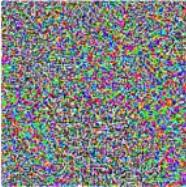
\includegraphics[height=0.5\textheight]{zy.jpg}
		\end{figure}
		\column{.3\textwidth}
		\begin{figure}
			\caption{What?}
			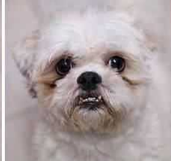
\includegraphics[height=0.5\textheight]{fig2.jpg}
		\end{figure}
		
	\end{columns}
	\begin{itemize}
		\item perturbations
	\end{itemize}
	
	
	
\end{frame}

\begin{frame}[fragile]{NonLinear}
	
	\begin{columns}[onlytextwidth]
		\column{1\textwidth}
		\begin{figure}

			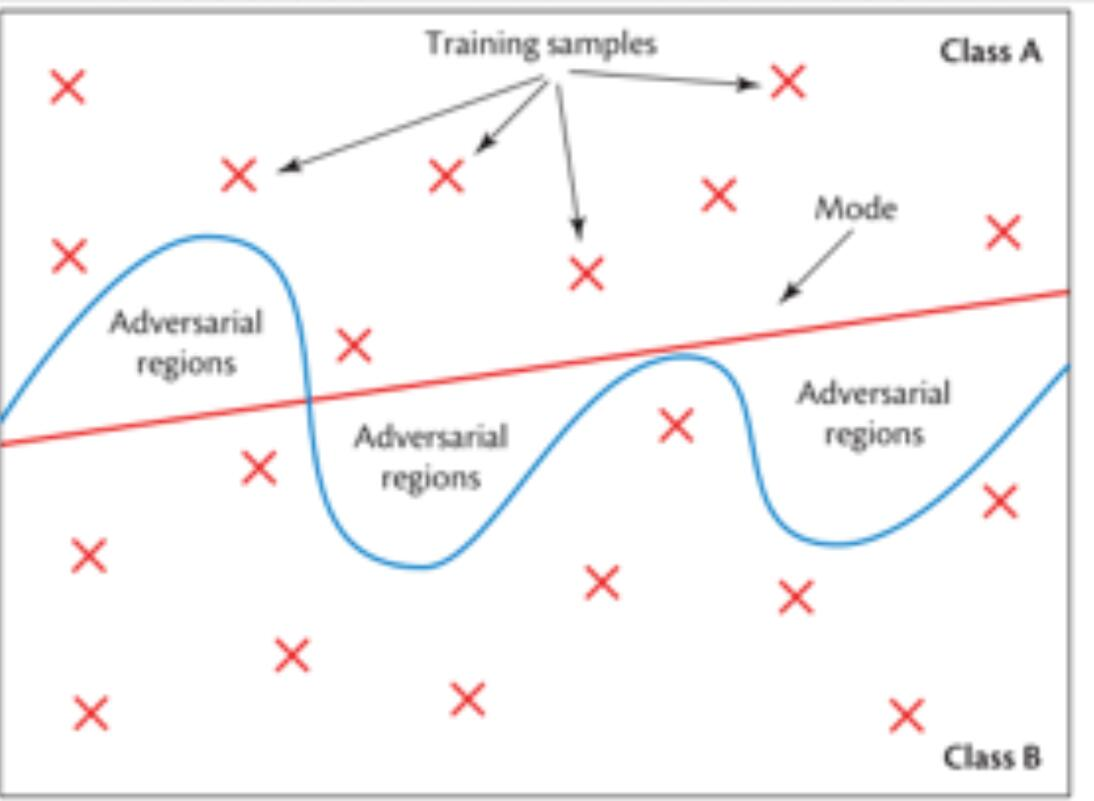
\includegraphics[height=.8\textheight]{exp1.jpg}
		\end{figure}

		
	\end{columns}
	
	
	
\end{frame}

\begin{frame}[fragile]{Linear Behavior}

\begin{itemize}
	\item The precision of an individual input feature is limited
	\item Example: 8 bits per pixel \& 1/255 of the dynamic
	range
	\item for the classifier to respond differently to an input $x$ than to an adversarial input $\widetilde{x}= x + \eta $ if every element of the perturbation $\eta$ is smaller than the precision of the features
	
\end{itemize}



\end{frame}



\section{Models}

\begin{frame}[fragile]{Models}
	\begin{columns}[onlytextwidth]
		\column{.8\textwidth}
		
		\begin{figure}
			%\caption{Dog}
			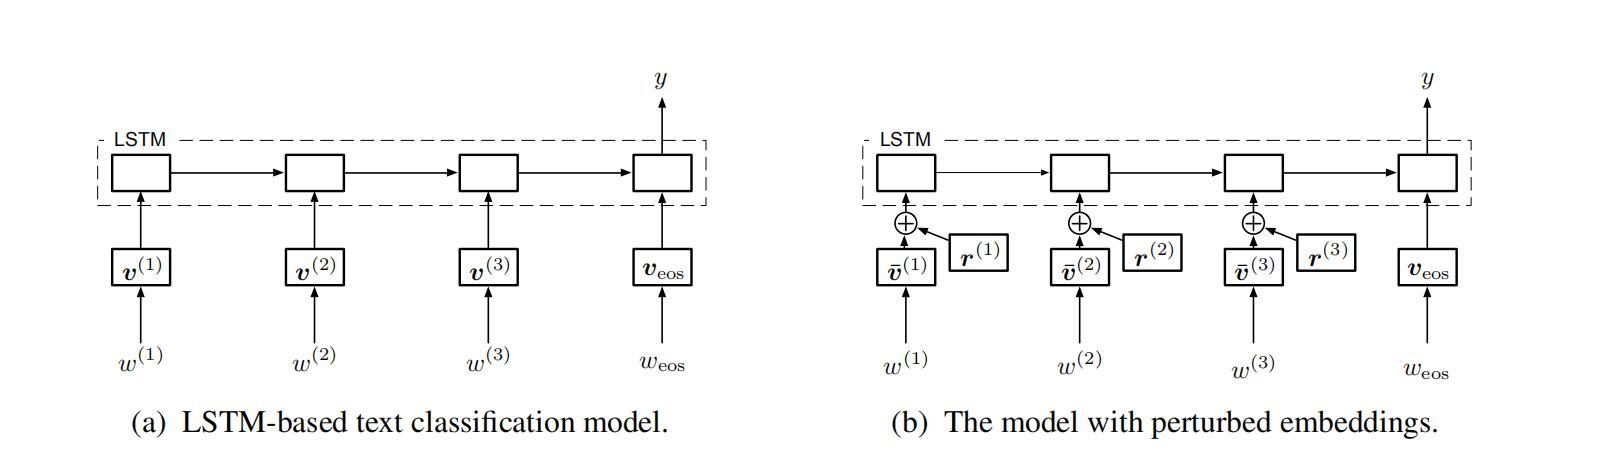
\includegraphics[height=0.5\textheight]{model.jpg}
		\end{figure}

		
	\end{columns}
	
	
\end{frame}
\section{Adversarial \& Virtual Adversarial Trianing}


\begin{frame}[fragile]{Symbols}

	\begin{table}[!htbp]
		\caption{ explanation of symbols}\label{tab:01} \centering
		\begin{tabular}{ccc}
			\toprule[1.5pt]
			symbol &  explanation of symbols\\ 
			\midrule[1pt]
			$x$ &  input vector \\
			$I$ &  input dimension \\
			$y$ &  labels \\
			$Q$ &  space of labels \\
			$p(y| x,\theta )$ & input probability distributions\\
			$D_l$ &  data with label\\
			$D_ul$ & data without label \\
			$\cdots$ & $\cdots$ \\
			\bottomrule[1.5pt]
		\end{tabular}
	\end{table}
	
\end{frame}

\begin{frame}[fragile]{Adversarial Training}
	\begin{itemize}
		\item loss function:
		\[
			L_{adv}:=D[q(y|x_l),p(y|x_l+r_{adv},\theta)] 
		\]
		\[	where\quad  r_{adv}:=arg\quad max_{r:\|r\|\leqslant \epsilon} \mathit{D}[q(y|x_l),p(y|x_l+r, \theta)]
		\]
		\item solution:
		\[
		 	r_{adv}\approx \epsilon\frac{g}{{\|g\|}^2},where \quad g=\nabla_{x_l}\mathit{D}[h(y;y_l),p(y|x_l, \theta)]
		\]
		\item or:
		\[
			r_{adv}\approx \epsilon \mathit{sign(g)}
		\]
	\end{itemize}
\end{frame}

\begin{frame}[fragile]{D? KL}
	\begin{itemize}
	\item Kullback–Leibler divergence
	\item How one probability distribution is different from a second.
	\end{itemize}

\end{frame}

\begin{frame}[fragile]{Kullback–Leibler divergence}
		\begin{columns}[onlytextwidth]
		\column{.7\textwidth}
		\begin{figure}
			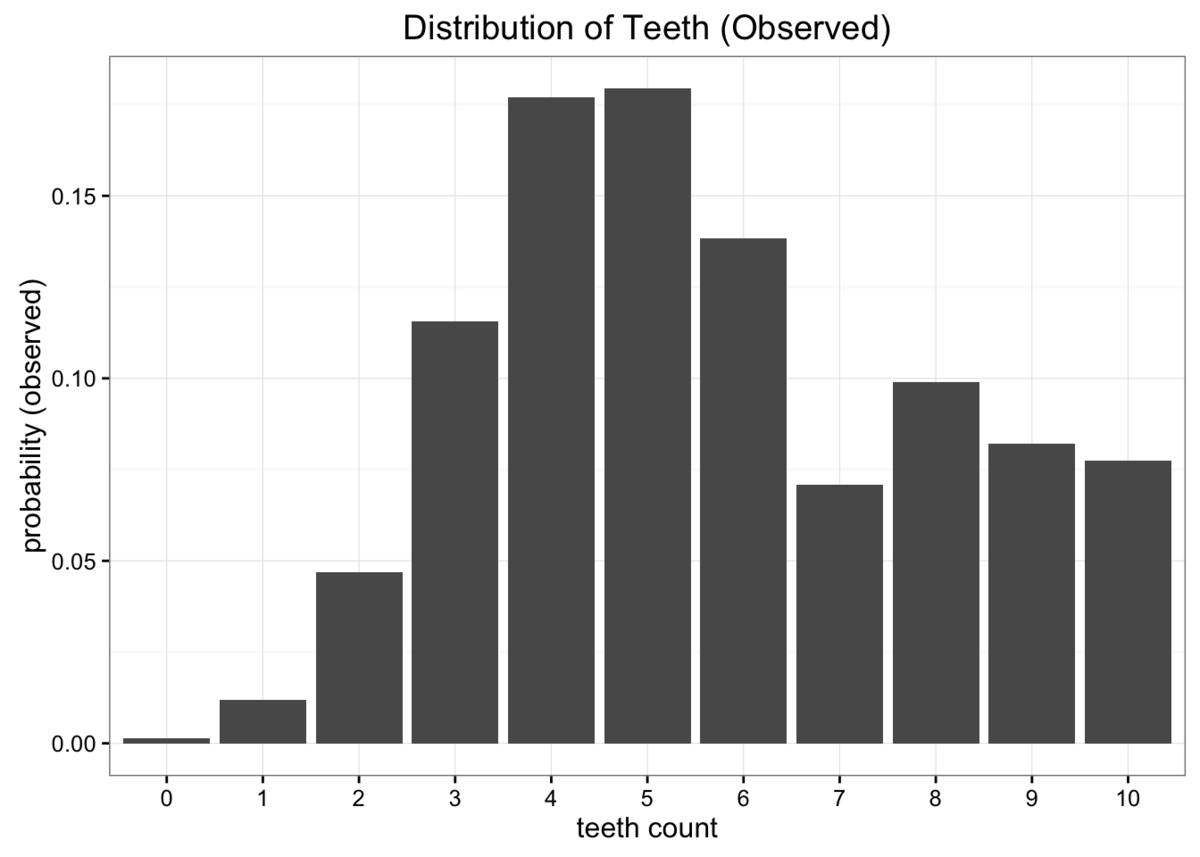
\includegraphics[height=0.8\textheight]{f1.png}
		\end{figure}
		\column{.4\textwidth}
		\begin{figure}
			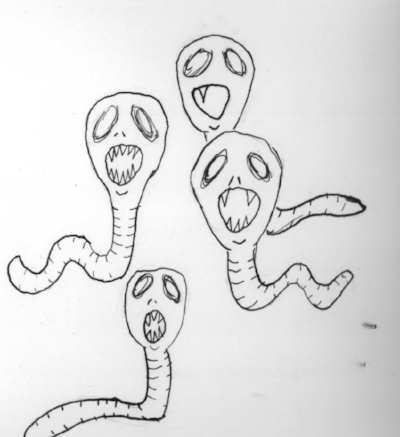
\includegraphics[height=0.5\textheight]{f2.png}
		\end{figure}

		
	\end{columns}
	
\end{frame}

\begin{frame}[fragile]{Kullback–Leibler divergence}
		\begin{columns}[onlytextwidth]
		\column{.3\textwidth}
		\begin{figure}

			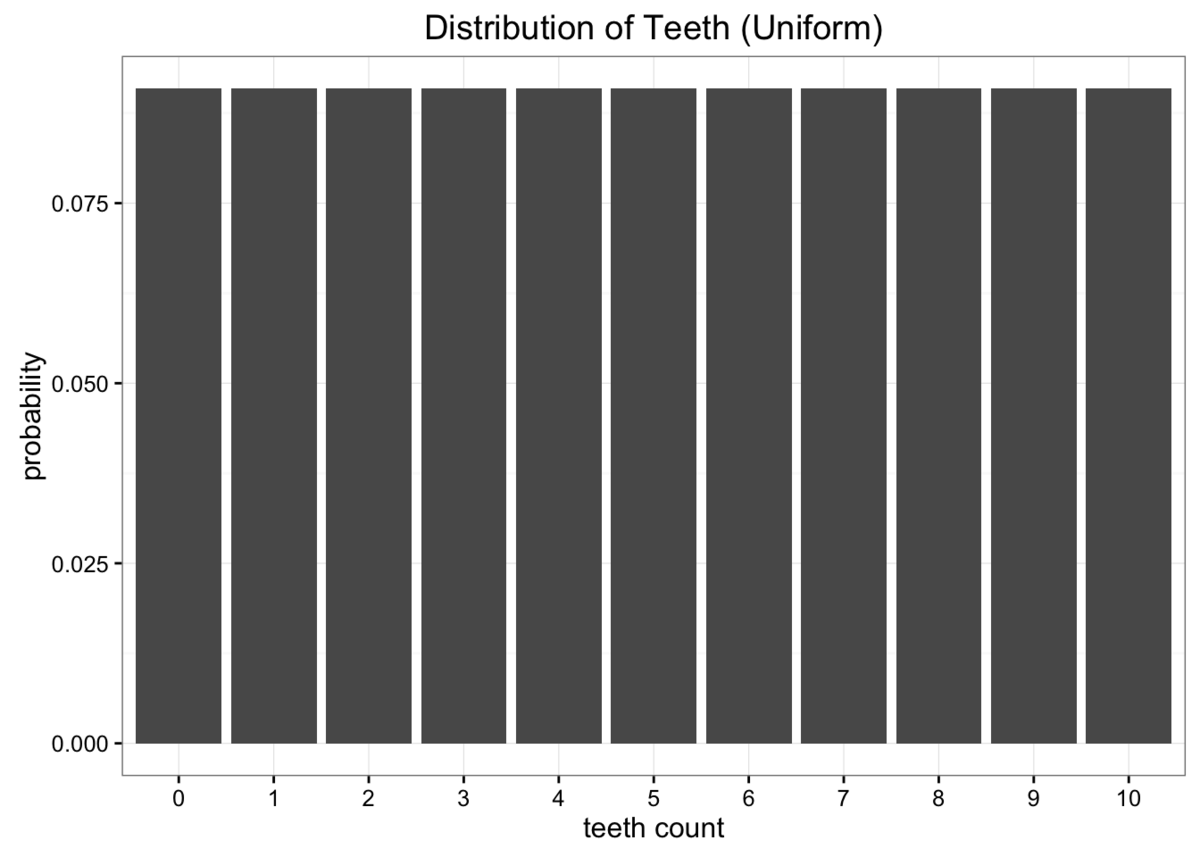
\includegraphics[height=0.5\textheight]{f3.png}
		\end{figure}
		\column{.3\textwidth}
		\begin{figure}

			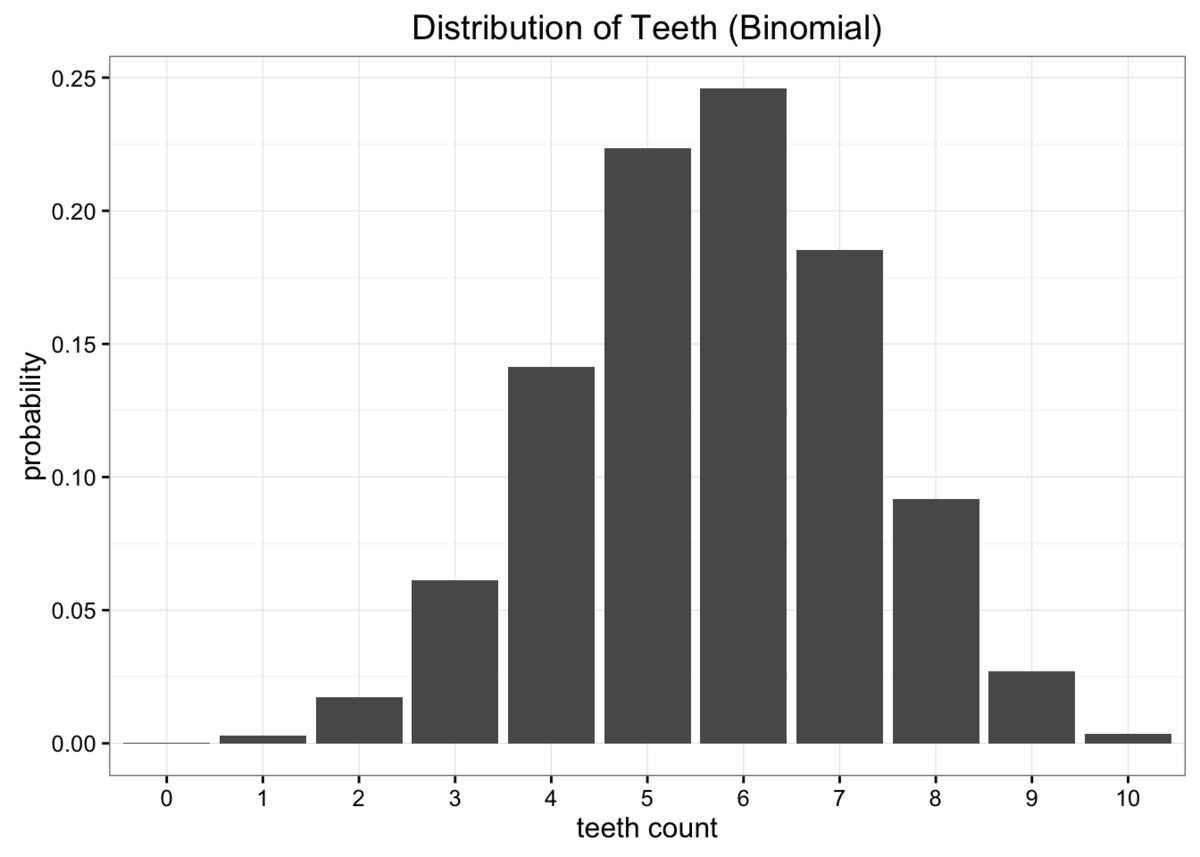
\includegraphics[height=0.5\textheight]{f4.png}
		\end{figure}
		\column{.3\textwidth}
		\begin{figure}

			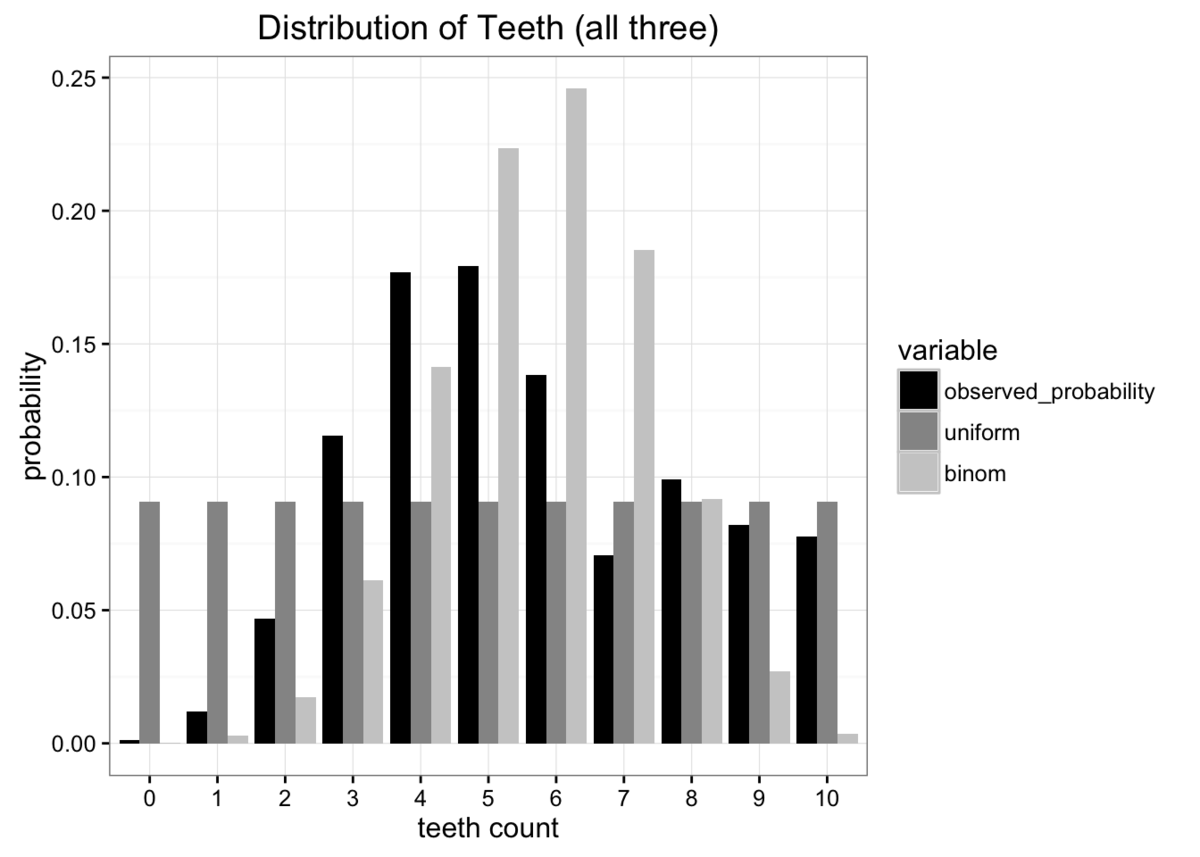
\includegraphics[height=0.5\textheight]{f5.png}
		\end{figure}
		
	\end{columns}
	
\end{frame}

\begin{frame}[fragile]{Adversarial Training}
	\begin{itemize}
		\item loss function:
		\[
		L_{adv}:=D[q(y|x_l),p(y|x_l+r_{adv},\theta)] 
		\]
		\[	where\quad  r_{adv}:=arg\quad max_{r:\|r\|\leqslant \epsilon} \mathit{D}[q(y|x_l),p(y|x_l+r, \theta)]
		\]
		\item solution:
		\[
		r_{adv}\approx \epsilon\frac{g}{{\|g\|}^2},where \quad g=\nabla_{x_l}\mathit{D}[h(y;y_l),p(y|x_l, \theta)]
		\]
		\item or:
		\[
		r_{adv}\approx \epsilon \mathit{sign(g)}
		\]
	\end{itemize}
\end{frame}

\begin{frame}[fragile]{VAT}
	\begin{itemize}
		\item target function:
		\[
		L_{qadv}:=D[q(y|x_*),p(y|x_*+r_{qadv},\theta)] 
		\]
		\[	where\quad  r_{qadv}:=arg\quad max_{r:\|r\|\leqslant \epsilon} \mathit{D}[q(y|x_*),p(y|x_*+r, \theta)]
		\]
		\item LDS and Regularization:
		\[
			\mathit{LDS(x_*},\theta):D[q(y|x_*,\widehat{\theta}),p(y|x_*+r_{qadv},\theta)]
		\]
		\[
		  where\quad  r_{qadv}:=arg\quad max_{r:\|r\|\leqslant \epsilon} \mathit{D}[q(y|x_*),p(y|x_*+r, \theta)]
		\]
		
 
	\end{itemize}
\end{frame}
\begin{frame}[fragile]{loss function}
	\[
	R_{vadv}(D_l,D_{ul},\theta):=\frac{1}{N_l+N_{ul}}\sum_{x_*\in D_L,D_{ul}}^{}LDS(x_*,\theta)
	\]
	\[
		\mathit{loss}=l(D_l,\theta)+\alpha R_{vadv}(D_l,D_{ul},\theta)
	\]
	
	
\end{frame}



\begin{frame}{Algorithm }
	\LinesNumberedHidden
	\begin{algorithm}[H]
		\label{1}
		\caption{Mini-batch SGD for $\nabla_\theta R_{vadv}(\theta)|_\theta=\widehat{\theta}$,\quad with a one-time power iteration method }
		(1) Choose M samples of $x^{(i)}(i=1,\cdots,M)$from dataset $D$ at random.\\
		(2) Generate a random unit vector $d^{(i)}\quad in\quad R^I$ using an iid Gaussian distribution.\\
		(3) Calculate $r_{vadv}$ via taking the gradient of $D$ with respect to $r$ on $r=\xi d^{(i)}$ on each input data point $x^{(i)}$:
		\[
		g^{(i)} \gets \nabla_r D[p(y|x^{(i)},\widehat{\theta}),p(y|x^{(i)}+r,\widehat{\theta})]|_{r=\xi d^{(i)}}
		\]
		\[
		r_{vadv}^{(i)} \gets g^{(i)} / \| g^{(i)} \| _2
		\]
		(4)Return $\nabla_\theta(\frac{1}{M}\sum_{i=1}^{M}\mathit{D}[p(y|x^{(i)},\widehat{\theta}),p(y|x^{(i)}+r,\widehat{\theta})])$
		
	\end{algorithm}
\end{frame}



\section{Experiment and Conclusion}

\begin{frame}{Dataset}
\begin{columns}[onlytextwidth]

		\column{1.2\textwidth}
		\begin{figure}
			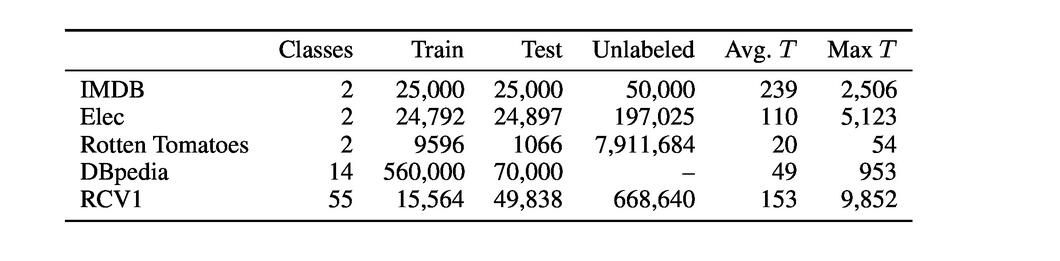
\includegraphics[width=.9\linewidth]{dataset.jpg}
		\end{figure}
	\end{columns}
\end{frame}

\begin{frame}{No Overfit}
	\begin{columns}[onlytextwidth]
		
		\column{1.2\textwidth}
		\begin{figure}
			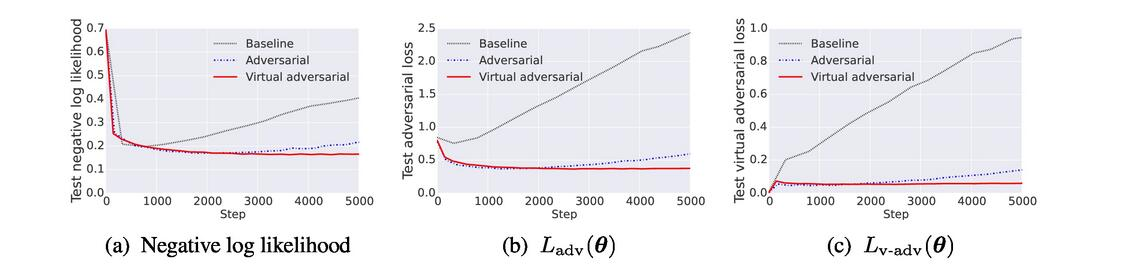
\includegraphics[width=.9\linewidth]{quxian.jpg}
		\end{figure}
	\end{columns}
\end{frame}

\begin{frame}{Result to IMDB}
	\begin{columns}[onlytextwidth]
		
		\column{.9\textwidth}
		\begin{figure}
			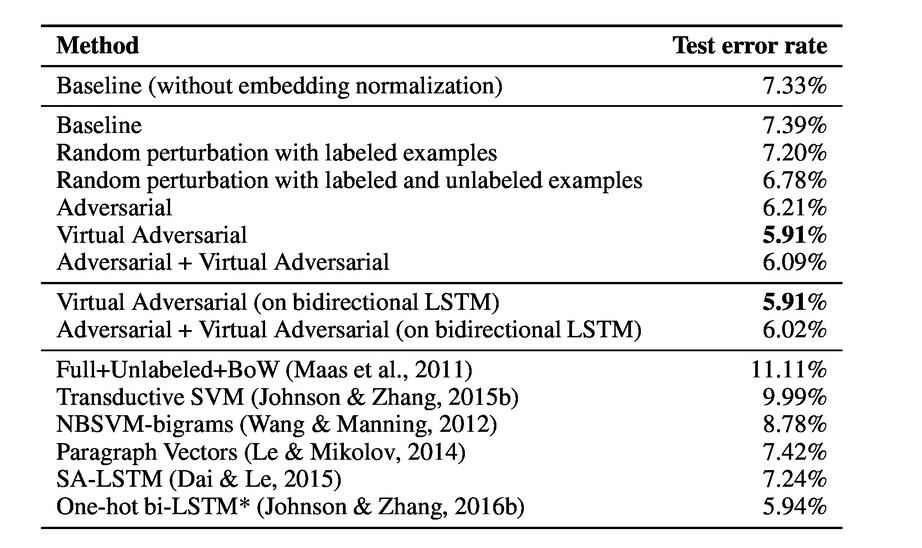
\includegraphics[width=.9\linewidth]{imdb.jpg}
		\end{figure}
	\end{columns}
\end{frame}

\begin{frame}{Good or Bad?}
	\begin{columns}[onlytextwidth]
		
		\column{1\textwidth}
		\begin{figure}
			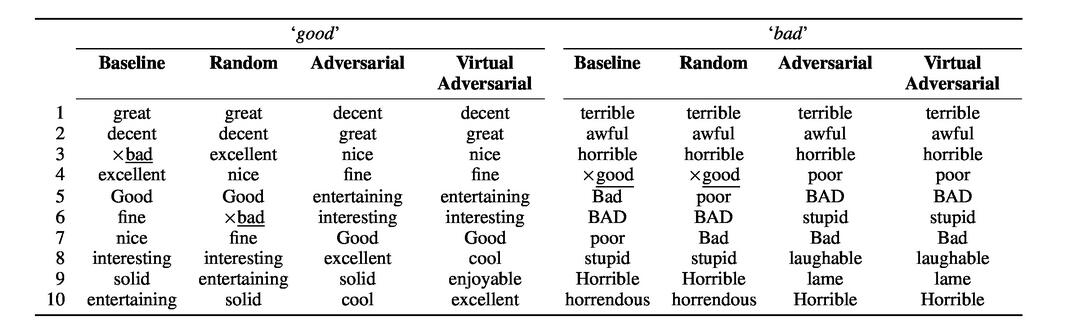
\includegraphics[width=1\linewidth]{goodbad.jpg}
		\end{figure}
	\end{columns}
\end{frame}

\begin{frame}{Results on Elec and RCV1}
	\begin{columns}[onlytextwidth]
		
		\column{1\textwidth}
		\begin{figure}
			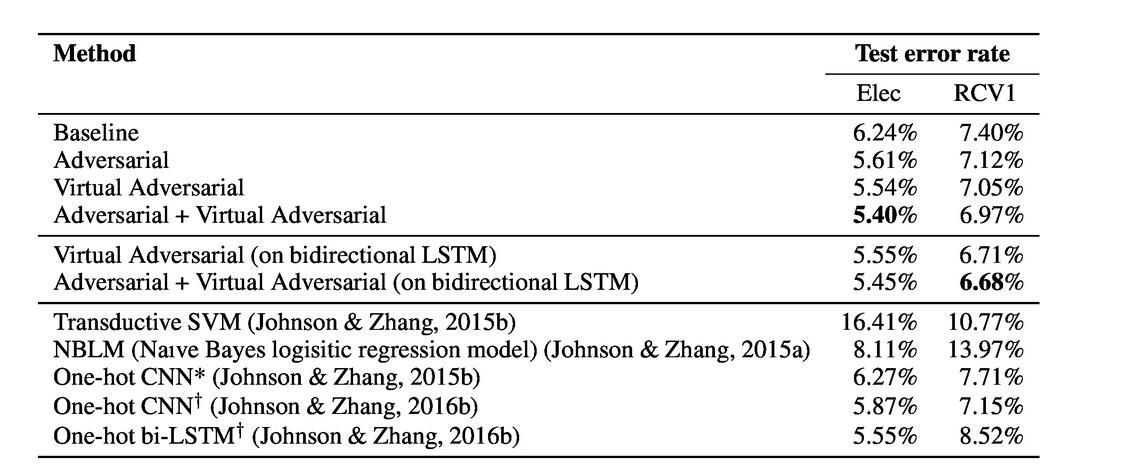
\includegraphics[width=1\linewidth]{elec.jpg}
		\end{figure}
	\end{columns}
\begin{itemize}
	\item $*$ indicates using pretrained embeddings of CNN, and $\dag$ indicates using pretrained embeddings of CNN and bidirectional LSTM
	\end{itemize}
\end{frame}

\begin{frame}{Thanks to \LaTeX\quad and mtheme}
	
	Get the source of this theme and the demo presentation from
	
	\begin{center}\url{github.com/matze/mtheme}\end{center}
	
	The theme \emph{itself} is licensed under a
	\href{http://creativecommons.org/licenses/by-sa/4.0/}{Creative Commons
		Attribution-ShareAlike 4.0 International License}.
	
	\begin{center}\ccbysa\end{center}
	
\end{frame}

\begin{frame}{OpenSource}
	
	Get the source code of this slide from
	
	\begin{center}\url{github.com/lwshanbd/bigdata_slide}\end{center}
	

	
\end{frame}
\input{conclusion.tex}

\begin{frame}[standout]
  Questions?
\end{frame}

\begin{frame}[standout]
  Thanks.
\end{frame}

\end{document}